\documentclass[../../../../main.tex]{subfiles}

\begin{document}

\section*{京都大学 1983年 前期}

\begin{center}
\begin{tabular}{|c|l|c|c|c|}
\hline
\multicolumn{2}{|c|}{} & 計 & 思 & 総 \\
\hline
1 & 確率 \quad $\star$ & B & C & B \\
\hline
3 & 多変数 & B & C & B \\
\hline
2 & 行列 & \multirow{2}{*}{B} & \multirow{2}{*}{B} & \multirow{2}{*}{B} \\
\cline{1-2}
4 & 空間 & & & \\
\hline
5 & 多変数 \quad $\star$ & C & B & B \\
\hline
6 & 多変数 \quad $\star$ & B & B & B \\
\hline
\end{tabular}
\end{center}

\subsection*{第1問}
[解] $A, B, C$の勝つ確率は右図のようである。\\
\begin{minipage}{0.4\textwidth}
\begin{tabular}{|c|c|c|c|}
\hline
相手 & A & B & C \\
\hline
A & \diagbox{}{} & $p$ & $q$ \\
\hline
B & $1-p$ & \diagbox{}{} & $\frac{1}{2}$ \\
\hline
C & $1-q$ & $\frac{1}{2}$ & \diagbox{}{} \\
\hline
\end{tabular}
\end{minipage}

(1) もとめる確率を$P_a$とする。右図から、
\[ P_a = pq + p(1-q) \cdot \frac{1}{2} \cdot P_a \]
\[ \therefore P_a = \frac{2pq}{2-p(1-q)} \]

\begin{tikzpicture}[x=0.5cm, y=-0.5cm, baseline=(current bounding box.north)]
\node at (0,0) {A};
\node at (2,0) {B};
\node at (4,0) {C};
\node at (6,0) {B};
\node at (8,0) {A};
\draw (0,0.5) -- (0,1) -- (2,1) -- (2,0.5);
\draw (1,1) -- (1,1.5) -- (4,1.5) -- (4,0.5);
\draw (2.5,1.5) -- (2.5,2) -- (6,2) -- (6,0.5);
\draw (4.25,2) -- (4.25,2.5) -- (8,2.5) -- (8,0.5);
\draw[dashed] (6.125,2.5) -- (6.125,3.5);
\end{tikzpicture}

(2) もとめる確率を$P_b$とする。右図から、
\[ P_b = (1-p) \frac{1}{2} \cdot P_c \]
$P_c$は(1)で$p$と$q$を入れかえたものだから、
\[ P_b = \frac{pq(1-p)}{2-q(1-p)} \]

\begin{tikzpicture}[x=0.5cm, y=-0.5cm, baseline=(current bounding box.north)]
\node at (0,0) {A};
\node at (2,0) {B};
\node at (4,0) {C};
\node at (6,0) {A};
\draw (0,0.5) -- (0,1) -- (2,1) -- (2,0.5);
\draw (1,1) -- (1,1.5) -- (4,1.5) -- (4,0.5);
\draw (2.5,1.5) -- (2.5,2) -- (6,2) -- (6,0.5);
\draw[dashed] (4.25,2) -- (4.25,3);
\node[right] at (4.5, 3) {これ以降Aが優勝する確率が $P_c$ となる。};
\end{tikzpicture}

(3) もとめる確率を$R$とする。1回目でどちらが勝つかで場合分けして、
\[ R = \frac{1}{2} (P_a + P_c) = pq \left\{ \frac{1}{2-p(1-q)} + \frac{1}{2-q(1-p)} \right\} \]

\subsection*{第2問}
[解]\\
$BC : \frac{x}{b} + \frac{y}{c} = 1$\\
$l : b(x-b) - cy = 0$\\
$m : bx - c(y-c) = 0$\\
だから、$P(bX, cY)$ とおくと ($X+Y=1$)\\
$Q\left(bX, \frac{b^2}{c}(X-1)\right), R\left(\frac{c^2}{b}(Y-1), cY\right)$\\
だから $X+Y=1$ から
\[ \overrightarrow{AQ} = \begin{pmatrix} bX \\ -\frac{b^2}{c}Y \end{pmatrix}, \overrightarrow{AR} = \begin{pmatrix} -\frac{c^2}{b}X \\ cY \end{pmatrix} \]
となり、$\overrightarrow{AQ} \parallel \overrightarrow{AR}$ だから、$Q, R, A$ は一直線上にある (図)\\

\begin{tikzpicture}
\draw[->] (-1,0) -- (4,0) node[right] {$x$};
\draw[->] (0,-1) -- (0,3) node[above] {$y$};
\coordinate (A) at (0,0);
\coordinate (B) at (3,0);
\coordinate (C) at (0,2);
\coordinate (P) at (1.5,1);
\coordinate (Q) at (1.5,-1.125);
\coordinate (R) at (-2,1);

\draw (B) -- (C);
\node[below left] at (A) {A};
\node[below] at (B) {B};
\node[left] at (C) {C};
\node[above right] at (P) {P};

\draw[dashed] (P) -- (Q);
\draw[dashed] (P) -- (R);
\node[below] at (Q) {Q};
\node[left] at (R) {R};
\draw (B) -- (1.5, -1.125) node[midway, right] {$l$};
\draw (C) -- (-2, 1) node[midway, above] {$m$};
\end{tikzpicture}

(2) 図のように定めると、題意の時
\[ \frac{1}{2} (\alpha + \gamma) \cdot h = 2 \cdot \frac{1}{2} \beta h \]
\[ \alpha + \gamma = 2\beta \quad \cdots \text{①} \]
である。

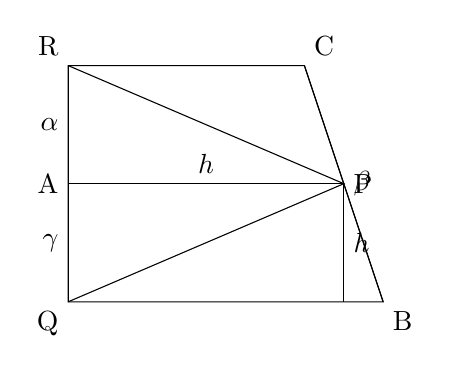
\begin{tikzpicture}
\coordinate (R) at (0,3);
\coordinate (C) at (3,3);
\coordinate (A) at (0,1.5);
\coordinate (Q) at (0,0);
\coordinate (B) at (4,0);
\coordinate (P) at (3.5, 1.5);

\draw (R) -- (C) -- (B) -- (Q) -- cycle;
\draw (R) -- (P) -- (Q);
\draw (C) -- (P) -- (B);
\draw (A) -- (P);

\node[above left] at (R) {R};
\node[above right] at (C) {C};
\node[left] at (A) {A};
\node[below left] at (Q) {Q};
\node[below right] at (B) {B};
\node[right] at (P) {P};

\node[left] at (0, 2.25) {$\alpha$};
\node[left] at (0, 0.75) {$\gamma$};
\node[right] at (3.5, 1.5) {$\beta$};

\draw (P) -- (0, 1.5) node[midway, above] {$h$};
\draw (P) -- (3.5, 0) node[midway, right] {$h$};
\end{tikzpicture}

\begin{itemize}
\item[$1^\circ$] $\text{RQ} \not\parallel \text{BC}$ の時\\
①なら AはRQの中点であり（ $\because$ \\
$|AQ|^2 = |AR|^2$\\
$\iff b^2 X^2 + \frac{b^4}{c^2} Y^2 = c^2 Y^2 + \frac{c^4}{b^2} X^2$\\
$\iff \frac{b^4 - c^4}{c^2} Y^2 = \frac{c^4 - b^4}{b^2} X^2$\\
$\iff \frac{Y^2}{c^2} = -\frac{X^2}{b^2} \quad (\because b \neq c)$\\
となり、$b, c, X, Y \in \mathbb{R}$, $X+Y=1$ に矛盾。よってこの時①のようにはならない

\item[$2^\circ$] $\text{RQ} \parallel \text{BC}$ の時\\
AはRQ上の任意の点で①をみたす（ $\because X = \frac{b^2}{b^2+c^2} \quad (0 < \frac{b^2}{b^2+c^2} < 1)$ となれば、$\overrightarrow{AQ} \parallel \overrightarrow{BC}$ となって適する）\\
以上から①のようになるのは $\text{RQ} \parallel \text{BC}$ の時で、この時、題意から\\
$\square \text{BCRQ} \text{は長方形}$\\
である。
\end{itemize}

\subsection*{第3問}
% 空白

\subsection*{第4問}
[解]\\
(1)\\
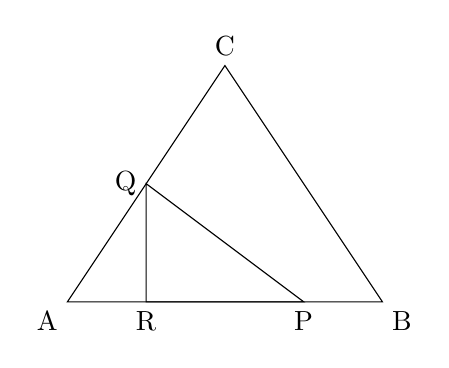
\begin{tikzpicture}
\coordinate (A) at (0,0);
\coordinate (B) at (4,0);
\coordinate (C) at (2,3);
\draw (A) -- (B) -- (C) -- cycle;
\coordinate (R) at (1,0);
\coordinate (P) at (3,0);
\coordinate (Q) at (1,1.5);
\draw (Q) -- (P) -- (R) -- cycle;
\node[below left] at (A) {A};
\node[below right] at (B) {B};
\node[above] at (C) {C};
\node[below] at (R) {R};
\node[below] at (P) {P};
\node[left] at (Q) {Q};
\end{tikzpicture}
\begin{tikzpicture}
\coordinate (O) at (0,0);
\coordinate (A) at (3,0);
\coordinate (B) at (0,3);
\coordinate (C) at (1.5,1.5);
\draw (O) -- (A) node[midway, below] {$a$};
\draw (O) -- (B) node[midway, left] {$b$};
\draw (O) -- (C) node[midway, right] {$c$};
\draw (A) -- (B) -- (C) -- cycle;
\node[below left] at (O) {O};
\node[right] at (A) {A};
\node[above] at (B) {B};
\node[above right] at (C) {C};
\end{tikzpicture}

底面を各々$\triangle ABC, \triangle PQR$とみると、高さ一定だから
\[ V_{OPQR} : V_{OABC} = \triangle PQR : \triangle ABC \quad \cdots \text{①} \]
である。三角形の相似から
\[ \overline{AQ} : \overline{AO} = a : \sqrt{a^2+c^2} \therefore \overline{AQ} = \frac{a^2}{\sqrt{a^2+c^2}} \]
同様にして
\[ \overline{AR} = \frac{a^2}{\sqrt{a^2+b^2}}, \quad \overline{BP} = \frac{b^2}{\sqrt{b^2+c^2}} \]
だから $\triangle ABC$の面積を1として
\begin{align*}
\triangle ARQ &= \frac{a^2}{a^2+b^2} \cdot \frac{a^2}{a^2+c^2} \\
\triangle BPR &= \frac{b^2}{a^2+b^2} \cdot \frac{b^2}{b^2+c^2} \\
\triangle PCQ &= \frac{c^2}{b^2+c^2} \cdot \frac{c^2}{a^2+c^2}
\end{align*}
だから
\begin{align*}
\triangle PQR &= 1 - \frac{a^4(b^2+c^2) + b^4(c^2+a^2) + c^4(a^2+b^2)}{(a^2+b^2)(b^2+c^2)(c^2+a^2)} \\
&= \frac{2a^2b^2c^2}{(a^2+b^2)(b^2+c^2)(c^2+a^2)}
\end{align*}
より ①から
\[ V_{OPQR} : V_{OABC} = 2a^2b^2c^2 : (b^2+c^2)(c^2+a^2)(a^2+b^2) \]

(2) (1)から
\[ \frac{2a^2b^2c^2}{(b^2+c^2)(c^2+a^2)(a^2+b^2)} \le \frac{1}{4} \]
\[ 8ABC \le (B+C)(C+A)(A+B) \quad \cdots \text{②} \]
($A=a^2, B=b^2, C=c^2$ とおいた)\\
を示せばよい。A,B,CからAM-GMより
\[ B+C \ge 2\sqrt{BC} > 0 \]
などとした3式をかけあわせると ②は示される(終)

\subsection*{第5問}
[解] 到達時刻 $t_0$ とする。右のように点 P, Q を定める。
\[ |\overline{OP}| = |t-a|, \quad |\overline{OQ}| = |t_0-b|, \quad |\overline{PQ}| = \sqrt{2}(t_0-t) \]
だから、$\triangle OPQ$ にピタゴラスの定理を用いて、
\[ 2(t_0-t)^2 = (t-a)^2 + (t_0-b)^2 \quad \cdots \text{①} \]

\begin{tikzpicture}
\draw[->] (-1,0) -- (4,0) node[right] {$x$};
\draw[->] (0,-1) -- (0,4) node[above] {$y$};
\coordinate (O) at (0,0);
\coordinate (P) at (2,0);
\coordinate (Q) at (0,3);
\draw (P) -- (Q);
\node[below left] at (O) {O};
\node[below right] at (P) {P};
\node[above left] at (Q) {Q};
\node[below] at (2,-0.2) {$t-a$};
\node[left] at (-0.2,3) {$t_0-b$};
\node[above right] at (1,1.5) {$\sqrt{2}(t_0-t)$};
\end{tikzpicture}

$S = t_0 - t$ とすると、$S$ を min にする $t$ をもとめれば良い。①に代入して
\begin{align*}
2 S^2 &= (t-a)^2 + (S + t - b)^2 \\
&= S^2 + 2(t-b)S + (t-b)^2 + (t-a)^2
\end{align*}
\[ \therefore S^2 - 2(t-b)S - (t-a)^2 - (t-b)^2 = 0 \]
\[ \therefore S = t-b + \sqrt{2(t-b)^2 + (t-a)^2} \quad (\because S > 0) \]
であるから、両辺 $t$ で微分して、
\[ \frac{dS}{dt} = 1 + \frac{2(t-b) + (t-a)}{\sqrt{2(t-b)^2 + (t-a)^2}} \]
だから、
\[ \frac{dS}{dt} \ge 0 \iff \sqrt{2(t-b)^2 + (t-a)^2} \ge -2(t-b) - (t-a) \]
$-2(t-b) - (t-a) \ge 0 \iff t \le \frac{a+2b}{3}$ のもとで2乗して解く（$t \ge \frac{a+2b}{3}$ のときは常に $\frac{dS}{dt} \ge 0$ ）
\begin{align*}
2(t-b)^2 + (t-a)^2 &\ge 4(t-b)^2 + (t-a)^2 + 4(t-a)(t-b) \\
\iff 0 &\ge 2(t-b)^2 + 4(t-b)(t-a) \\
&= 2(t-b) \{ 3t - (2a+b) \} \\
\iff \frac{2a+b}{3} &\le t \le b \quad (\because 0 < a < b)
\end{align*}
だから、下表をうる。

\begin{center}
\begin{tabular}{|c|c|c|c|c|c|}
\hline
$t$ & $0$ & $\cdots$ & $\frac{2a+b}{3}$ & $\cdots$ & $b$ \\
\hline
$S'$ & & $-$ & $0$ & $+$ & \\
\hline
$S$ & & $\searrow$ & & $\nearrow$ & \\
\hline
\end{tabular}
\end{center}
したがって、もとめるのは $t = \frac{2a+b}{3}$ である。

\subsection*{第6問}
[解] 時刻 $t$ での水面の面積 $P$ とすると、
\[ -S v = P \frac{dx}{dt} \quad \cdots \text{①} \]
ここで、
\[ P = \pi \left( \frac{x}{h} R \right)^2 = \frac{\pi R^2}{h^2} x^2 \quad \cdots \text{②} \]
及び
\[ v = k x \]
を①に代入して
\[ -S k x = \frac{\pi R^2}{h^2} x^2 \frac{dx}{dt} \]
$x > 0$ より、
\[ -S k = \frac{\pi R^2}{h^2} x \frac{dx}{dt} \]
両辺積分して、$t = 0$ で $x = h$ より、
\[ -S k t + \frac{1}{2} \pi R^2 = \frac{1}{2} \frac{\pi R^2}{h^2} x^2 \]
$x > 0$ より、
\[ x(t) = \sqrt{\frac{2h^2}{\pi R^2} \left( \frac{1}{2} \pi R^2 - Skt \right)} \]

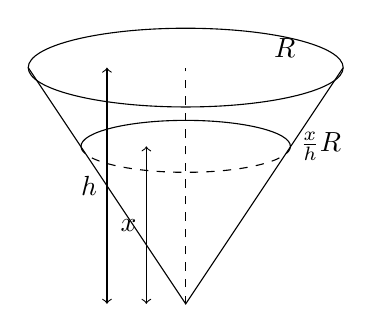
\begin{tikzpicture}
\draw (0,0) ellipse (2cm and 0.5cm);
\draw (-2,0) -- (0,-3) -- (2,0);
\draw[dashed] (0,-3) -- (0,0);
\draw[dashed] (-1.33,-1) arc (180:360:1.33cm and 0.33cm);
\draw (-1.33,-1) arc (180:0:1.33cm and 0.33cm);
\node[above right] at (1,0) {$R$};
\node[right] at (1.33,-1) {$\frac{x}{h}R$};
\draw[<->] (-0.5,-3) -- (-0.5,-1) node[midway, left] {$x$};
\draw[<->] (-1,-3) -- (-1,0) node[midway, left] {$h$};
\end{tikzpicture}

\end{document}
